\chapter{Conclusion}
\label{cap:conclusion}

Six years ago SDN and OpenFlow caused a stir in the world of computer networks. Although data and control plane separation is not a new idea, the flexibility and programmability enabled by OpenFlow started a wave of industry efforts to support the protocol in their products. Several OpenFlow 1.0 switches, controllers and test frameworks emerged from this movement, confirming the growing interest in this technology. Large networks operators, such as Google and Facebook, embraced OpenFlow interested in its potential. An organization, named Open Network Foundation, was created to speed up the OpenFlow development and adoption. Quickly, new versions of the protocol were released. This time, however, implementations did not arouse at the same time.

To keep up with the pace of the technology and to enable research capable of leveraging the new functionalities, we found the need to implement an OpenFlow 1.3 software switch. More than a full compliant implementation, requirements included minimal performance and ease of experimentation. This effort lead to the open source software implementation of the first OpenFlow 1.3 switch. 

Today, the software switch is a well known open source project and a cheap and friendly option to experiment OpenFlow 1.3. Although new software switches supporting OpenFlow 1.3 are now available, this work is still a solid and relevant option to prototype and develop new OpenFlow applications. In the next two sections, we present some significant obtained results and notorious use cases. Finally, we conclude this chapter discussing future areas for research and improvement in the software switch.     

\section{Results}
\label{sec:results}

In this section we list positive results achieved on the dissemination of our work:  

\begin{itemize}
\item \textbf{Development of an Open source community.} The choice of using GitHub to host the code proved to be a great way to reach a high number of users. Figure \ref{fig:ghstats}, shows information confirming the tool's popularity. In a 14 days interval, the software switch repository had 3125 accesses, with 796 unique visitors and cloned 97 times. 

When it comes to code contributions, there are 15 users listed in GitHub that submitted pull requests. Also, there is a number of contributors that send patches through other means.

This result is very important because the creation of a community around open source code gives it visibility, helps to spread the software and speed up reports of detected bugs. 

\begin{figure}[H]
\centering
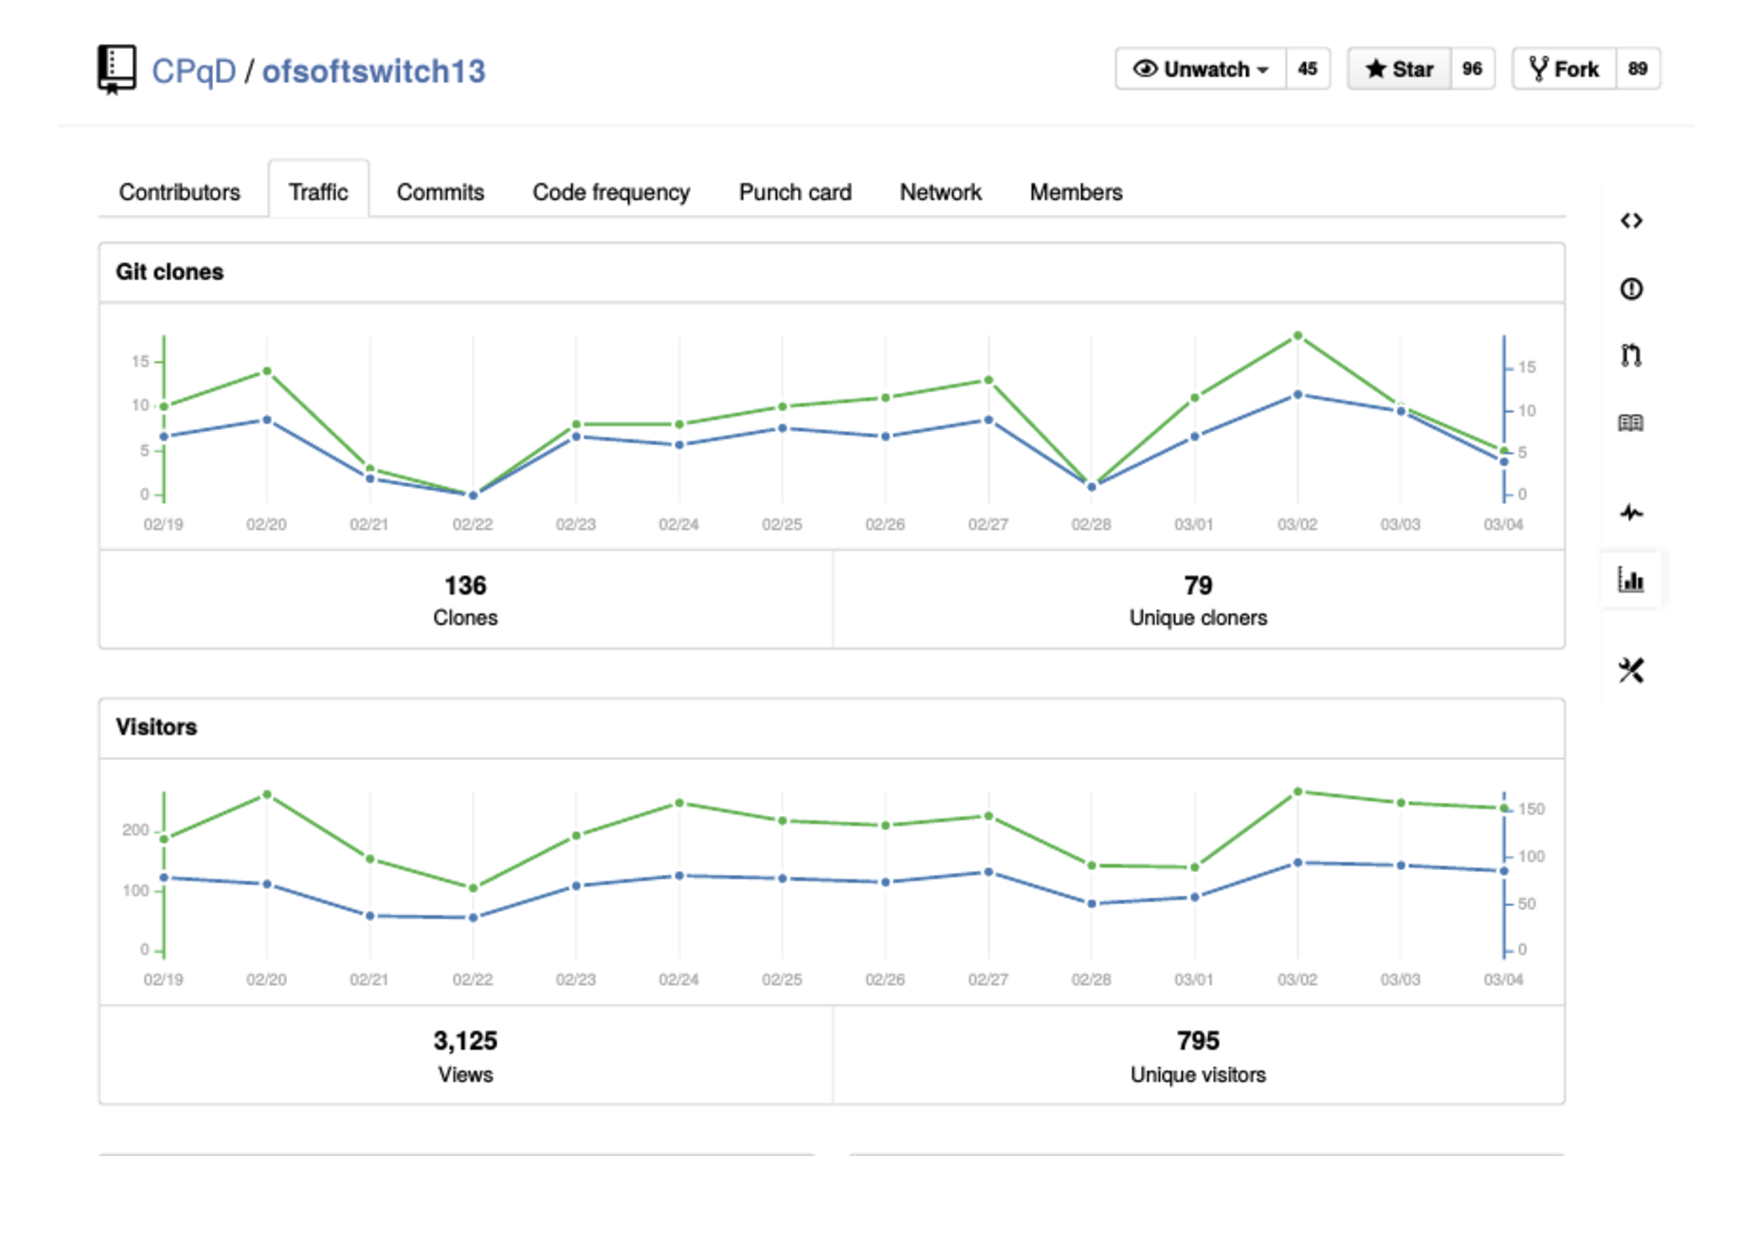
\includegraphics[height=20cm,width=\textwidth,keepaspectratio]{eps/GH.pdf}
\caption{GitHub statistics.}
\label{fig:ghstats}
\end{figure}

\item \textbf{Part of Mininet installation options.} The software switch is included among the installation options of Mininet. It makes easier for users to start experimenting with OpenFlow 1.3. Another great effect is the numbers of users reached, since this work is the default OpenFlow 1.3 userspace switch in Mininet.      

\item \textbf{Publications.} This work gave origin to three publications. The first paper is about IPv6 support on OpenFlow. The second is an invited paper bringing perspectives on SDN for home network. These ideas were inspired by the software switch port to OpenWRT. Finally, the last paper is an overall presentation of this project, highlighting architectural and implementation details. These publications are listed on Annex \ref{AnnexB}.  
\end{itemize}


\section{Use Cases}
\label{sec:cases}

Known use cases show that the software is an important tool in the advance of the state of art on SDN research and development. As there is a large number of projects that are using or have made use of our work, we will list some notorious examples: 

\begin{itemize}
\item \textbf{Base for new OpenFlow features implementation.} The ONF group responsible by the addition of new OpenFlow features decided to publish new features only if properly implemented and tested. As OpenFlow 1.3 basic functionalities is required for 1.4 and 1.5, the Extensions Work Group chose our work as one of the software switches as a base to prototype new functionalities \cite{ONFproto}. 

\item \textbf{Academic.} The software switch has found good adoption by the academic community. For instance, works published in renowned conferences \cite{Reitblatt:2013:FDF:2491185.2491187} \cite{Bianchi:2014:OPP:2602204.2602211} and master dissertations \cite{Paris} \cite{ShahmirShourmasti656472} cite our software as the OpenFlow 1.3 switch chosen for their experiments.  

\item \textbf{Industry.} Industrial development is harder to track because it is usually closed. However, one successful case is in the development of an application for the Open Network Operating System (ONOS). Built by two companies' teams, Dell and ON.Lab, the Segment Routing implementation used the software switch for its simplicity \cite{ONOS}.         
\end{itemize}

\section{Future Work}

Each architectural component from the software switch has space for improvements. New algorithms and data structures are objects of study for the Flow Table matching. More complex and precise algorithms for rate limiting might be considered for better Meter Table performance. As for groups, new bucket select types may be a subject for academic research. 

While there are open ideas for further research and development, some optimizations and features are planned for the software switch in the medium-term. These major improvements are listed below:

\begin{itemize}

\item \textbf{Support for OpenFlow 1.4 and 1.5}. OpenFlow 1.4 and 1.5 are extensions of OpenFlow 1.3 and it would be good to keep the pace with the OpenFlow evolution. Some OpenFlow 1.4 and 1.5 features are already implemented, as stated in section \ref{sec:cases}. However, we would like to have both versions supported in one single switch running instance, without need to split the code in two different programs.

\item \textbf{Hash based match.} Results found in experiments presented on section \ref{sec:bandflows} show a huge loss in performance due to linear matching. To solve this problem, flows entries might be represented as hash value into the Flow Table. Then, packet fields could also be turned into a hash and looked up in the Flow Table. This would give constant performance for the Flow Table look up. However, some relevant questions arise: 

    \begin{itemize}
    \item How to handle flow priority? Since flows should be matched in order of priority, how to ensure the first hash value for a flow is the one with higher priority? 
    \item How to deal with field masking? Some flow match fields may have a mask, so they should be considered in the hash calculation. The question is how to efficiently search and apply these masks to the packet hash calculation. 
    \end{itemize}

The search for an answer for these questions opens space for new research in OpenFlow and SDN, since these questions are not only related to the software switch. 
  
\item \textbf{New packet parsing engine}. The software switch relies on Netbee library to parse packets. While Netbee adds flexibility and extensibility for the parsing and the ease of addition of new protocols to OpenFlow, its code is neither frequently updated, nor following dependencies upgrades. This breaks the software switch compilation in more recent Linux versions, because of more recent versions of libraries required by Netbee. Due to the number of compilation issues related to Netbee, a new packet parsing module must replace the current third party library.

\end{itemize}

